\let\negmedspace\undefined
\let\negthickspace\undefined
\documentclass[journal]{IEEEtran}
\usepackage[a5paper, margin=10mm, onecolumn]{geometry}
%\usepackage{lmodern} % Ensure lmodern is loaded for pdflatex
\usepackage{tfrupee} % Include tfrupee package

\setlength{\headheight}{1cm} % Set the height of the header box
\setlength{\headsep}{0mm}     % Set the distance between the header box and the top of the text

\usepackage{gvv-book}
\usepackage{gvv}
\usepackage{cite}
\usepackage{amsmath,amssymb,amsfonts,amsthm}
\usepackage{algorithmic}
\usepackage{graphicx}
\usepackage{textcomp}
\usepackage{xcolor}
\usepackage{txfonts}
\usepackage{listings}
\usepackage{enumitem}
\usepackage{mathtools}
\usepackage{gensymb}
\usepackage{comment}
\usepackage[breaklinks=true]{hyperref}
\usepackage{tkz-euclide} 
\usepackage{listings}
% \usepackage{gvv}                                        
\def\inputGnumericTable{}                                 
\usepackage[latin1]{inputenc}                                
\usepackage{color}                                            
\usepackage{array}                                            
\usepackage{longtable}                                       
\usepackage{calc}                                             
\usepackage{multirow}                                         
\usepackage{hhline}                                           
\usepackage{ifthen}                                           
\usepackage{lscape}
\begin{document}

\bibliographystyle{IEEEtran}
\vspace{3cm}

\title{
7 - Circle \\
\large EE1030:Matrix Theory
}
\author{Gajjarapu Satyanarayana\\AI24BTECH11009
}
% \maketitle
% \newpage
% \bigskip
{\let\newpage\relax\maketitle}

\renewcommand{\thefigure}{\theenumi}
\renewcommand{\thetable}{\theenumi}



\numberwithin{equation}{enumi}
\numberwithin{figure}{enumi}
\renewcommand{\thetable}{\theenumi}


\textbf{Question}:7.2.23\\
If the lines $2x - 3y = 5$ and $3x - 4y = 7$ are the diameters of a circle of area 154 square units, then obtain the equation of the circle.
\\
\textbf{Solution:}
\renewcommand{\tablename}{Table 7.2.23.1}
\begin{table}[h!]
  \centering
  \begin{tabular}[12pt]{ |c| c|}
    \hline
    \textbf{Variables} & \textbf{Description}\\ 
    \hline
    $\textbf{V}_1, \vec{u}_1, f_1$ & Parameters of the parabola $y^2 = 4x$ \\
    \hline
     $\textbf{V}_2, \vec{u}_2, f_2$ & Parameters of the circle $4x^2 + 4xy^2 = 9$ \\
    \hline
    $\vec{x}^\intercal\brak{\textbf{V}_1 + \mu\textbf{V}_2}\vec{x} + 2\brak{\vec{u}_1 + \mu\vec{u}_2}^\intercal\vec{x} + \brak{f_1 + \mu f_2}$ & Intersection of two conics \\
    \hline
    \end{tabular}


  \caption{Variables and their description}
\end{table}
\\
The augmented matrix formed by the given equations of diameter is
\begin{align}
    \myvec{2 & -3 & 5 \\ 3 & -4 & 7} \xrightarrow[]{R_2 \rightarrow 2R_2 - 3R_1} & \myvec{2 & -3 & 5 \\ 0 & 1 & -1} \\
    \xrightarrow[]{R_1 \rightarrow R_1 + 3R_2} & \myvec{2 & 0 & 2 \\ 0 & 1 & -1} \\
    \xrightarrow[]{R_1 \rightarrow \frac{R_1}{2}} & \myvec{1 & 0 & 1 \\ 0 & 1 & -1} \label{eq7.2.23.1}
\end{align}
Therefore from equation \ref{eq7.2.23.1} centre of the circle is
\begin{align}
    \vec{c} & = \myvec{1 \\ -1} \\
    \vec{u} & = \myvec{-1 \\ 1} \\
    \vec{u}^\intercal & = \myvec{-1 & 1} \\
    \lVert\vec{u}\rVert^2 & = \vec{u}^\intercal \vec{u} \\
    \lVert\vec{u}\rVert^2 & = \myvec{-1 & 1}\myvec{-1 \\ 1} \\
    \lVert\vec{u}\rVert^2 & = 2
    \end{align}
Given area is 154 square units and taking $\pi$ = $\frac{22}{7}$ as approximation
\begin{align}
    \pi r^2 & = 154 \\
    r^2 & = 49 \\
    r & = 7 \\
    f & = 2 - 49 \\
    f & = -47
\end{align}
The equation of circle is given by
\begin{align}
    \lVert\vec{x}\rVert^2 + 2\vec{u}^\intercal\vec{x} + f & = 0 \\
    \vec{x}^\intercal\vec{x} + 2\myvec{-1 & 1}\vec{x} + (-47) & = 0 \\
    x^2 + y^2 - 2x + 2y - 47 & = 0
\end{align}
\begin{figure}[h!]
   \centering
   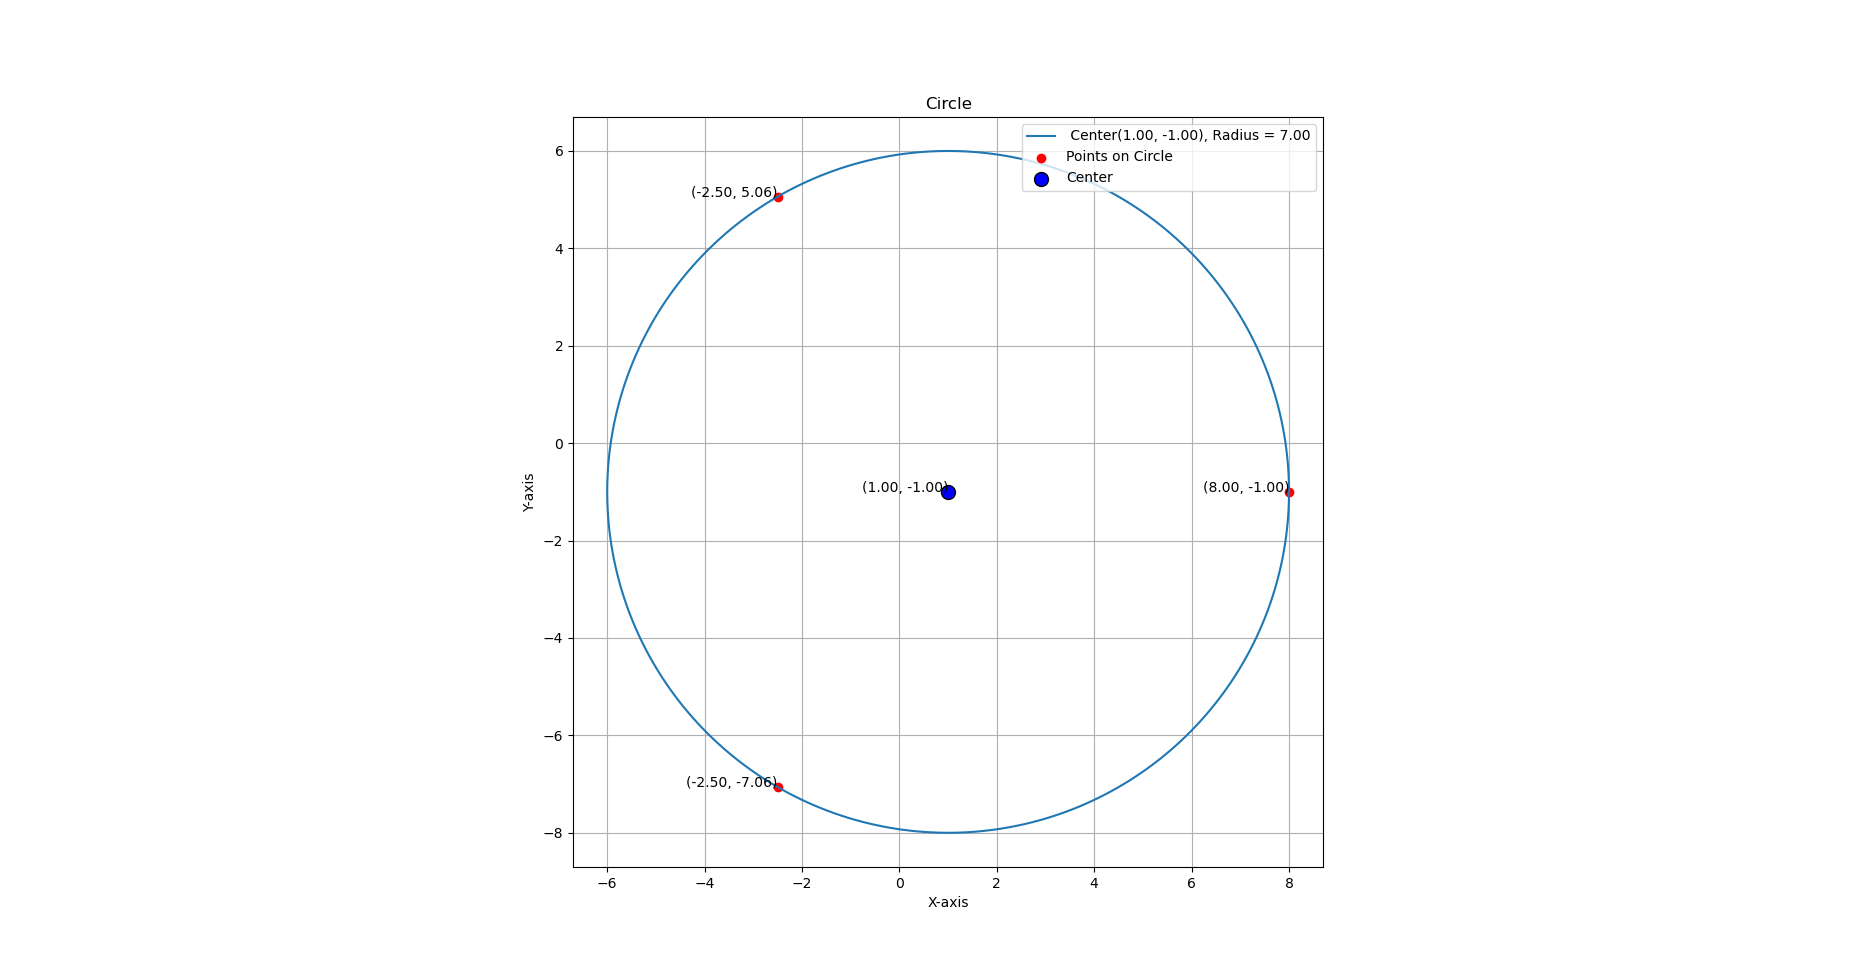
\includegraphics[width=0.9\linewidth]{figs/circle.png}
	\caption{Circle}
   \end{figure}
\end{document}

